\documentclass{article}

% Language setting
% Replace `english' with e.g. `spanish' to change the document language
\usepackage[english]{babel}

% Set page size and margins
% Replace `letterpaper' with `a4paper' for UK/EU standard size
\usepackage[letterpaper,top=2cm,bottom=2cm,left=3cm,right=3cm,marginparwidth=1.75cm]{geometry}

% Useful packages
\usepackage{amsmath}
\usepackage{graphicx}
\usepackage[colorlinks=true, allcolors=blue]{hyperref}

\usepackage{wrapfig}
\usepackage{mwe}


\title{ \Huge \textbf{Predicting Black Holes from Einstein's GR}}
\author{\large Riddhiman Bhattacharya}


\begin{document}
\maketitle



\begin{abstract}

\large

The presence of Black Holes was predicted by Albert Einstein through his groundbreaking theory of General Relativity in 1915[1]. Black Holes 
are the regions in space where gravity is extraordinarily strong where nothing, not even light can escape. 
The \textbf{Event Horizon/Schwarzschild Radius} represents the boundary beyond which nothing, including light, can escape the gravitational pull of a black hole.

According to the theory of general relativity, the Schwarzschild radius is the radius of a non-rotating black hole that has a mass M. It is defined by the equation:

$$R_s = \frac{2GM}{c^2}$$

where $R_s$ is the Schwarzschild radius, G is the gravitational constant, M is the mass of the black hole, and c is the speed of light in a vacuum.


Over the past century, numerous observational and theoretical studies have provided compelling evidence for the existence of these enigmatic cosmic objects [2]. In April 2019,  the Event Horizon Telescope (EHT) collaboration captured the first-ever image of a black hole's shadow.The image captured by the EHT was of the supermassive black hole at the center of the galaxy Messier 87 (M87). It provided visual evidence of the black hole's event horizon, confirming the existence of black holes and supporting the predictions of general relativity.
This overview provides a concise summary of our current understanding of black hole formation and the supporting evidence that stems from the predictions of general relativity. 
This article focuses on the remarkable connection between Sir Roger Penrose's discovery of black holes and the solid predictions made by the general theory of relativity. Specifically, we explore the singularity theorem, Penrose's seminal contribution to post-Einsteinian general relativity, which introduced the pivotal concept of a closed trapped surface.


\end{abstract}

\section{\Large Introduction}

\large 
The General Theory of Relativity(GR) by Albert Einstein is one of the most profound scientific theories of our time. This theory revolutionized our understanding of gravity, space-time, and has undergone extensive experimental validation. Among its intriguing predictions, the existence of black holes, objects of immense density, from which not even light can escape—has captivated scientists. While black holes were once considered purely theoretical, recent astronomical discoveries have unveiled objects in the cosmos that appear to be black holes.

\begin{figure}
    \centering
    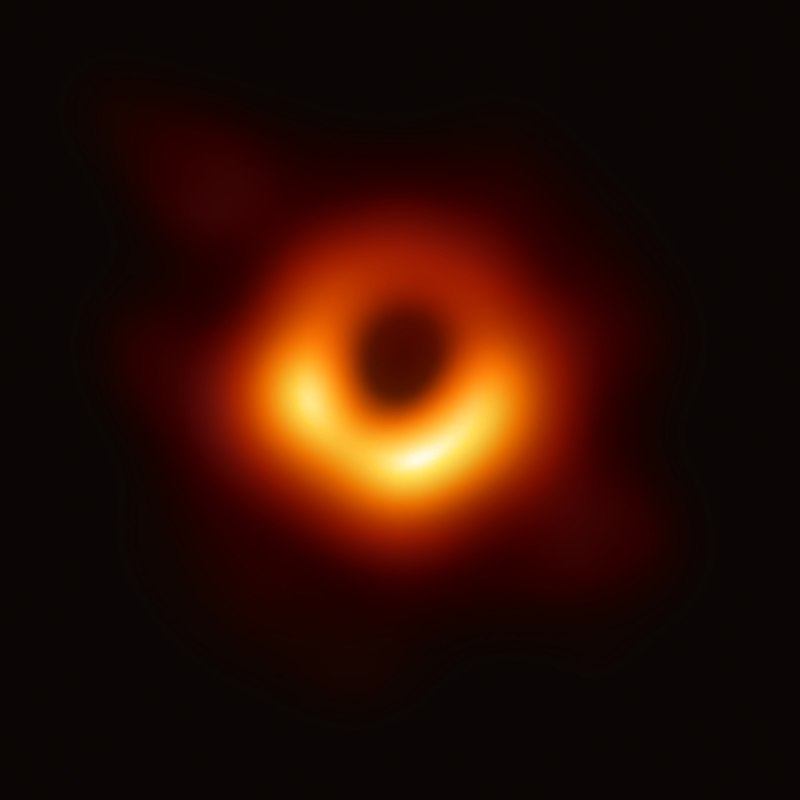
\includegraphics[width=0.5\textwidth]{BH-1.jpg}
    \caption{First Capture of Black Holes}
    \label{fig:1}
\end{figure}



Through computer simulations, scientists have explored the formation and evolution of black holes, confirming that their emergence is indeed a robust prediction of general relativity in various scenarios. Roger Penrose in his paper  "\textit{GRAVITATIONAL COLLAPSE AND SPACE-TIME SINGULARITIES }" introduced the concept of closed trapped surfaces, which has since become a fundamental idea in the study of black holes.
Through this paper we aim to examine the evidence supporting the formation of black holes as predicted by GR

\section{\Large Singularity}

\large 
In the realm of Lorentzian manifolds, a singularity refers to an irregular, unending curve [7, 8, 9, 10, 11, 12, 13]. While these curves may have finite values for their canonical parameters, they cannot be smoothly extended within spacetime. Consequently, \textit{singularity theorems establish only the existence of geodesic incompleteness, which is a necessary condition for singular spacetimes}. 

\section{\Large Discovery Method}

\large 
An essential aspect to understand the discovery of black holes is to understand the evolution of singularity theorem. The first singularity theorem was proposed by Amal Kumar Raychaudhur in 1955 and introduced the renowned equation later named after him [3]. Raychaudhuri investigated the possible paths taken by bundles of light rays in the curved regions of spacetime during the 1950s. The theorem's fundamental input, as highlighted by Raychaudhuri, was an equation derived from the Ricci identity that described this dynamical process. The well-known Raychaudhuri equation, as derived from the Ricci identity, is :

$$(\nabla_{\mu} \nabla_{\nu} - \nabla_{\nu} \nabla_{\mu}) u^{\alpha} = R_{\rho \mu \nu}^{\alpha} u^{\rho}$$

And now contracting $\alpha$ with $\mu$, the equation is simplified and given as follows:

$$u^\nu \nabla_{\mu} \nabla_{\nu} u^{\mu} - u^\nu \nabla_{\nu} \nabla_{\mu} u^\mu = R_{\rho v} u^{\rho} u^\nu $$



\section{\Large Penrose Singularity Theorem}

\large
Sir Roger Penrose made significant contributions to the study of black holes and singularities through his groundbreaking work on the Penrose Singularity Theorem. Unlike the traditional approach using spherical geometry, Penrose introduced the concept of trapped surfaces and utilized advanced geometry, specifically topology, to analyze the Einstein equations in contrast to the Schwarzschild solution [3].

Penrose's key insight was that if light cannot escape from a region, it is an indication that a singularity must form within that region. He demonstrated that the path of light will inevitably lead to the singularity in such cases. The event horizon of a black hole corresponds to this trapped surface, beyond which nothing, including light, can escape.
In the context of stellar collapse, Penrose showed that when the core of a massive star reaches a critical point and undergoes gravitational collapse, its intense gravity causes it to implode into an incredibly dense region. This collapse bends space-time indefinitely at the center and traps light within the event horizon, resulting in the formation of a black hole.


Penrose's singularity theorem established that under certain conditions, such as the presence of a non-compact Cauchy hypersurface and the satisfaction of convergence requirements, there will be future incomplete null geodesics associated with a closed future-trapped surface [1]. This theorem provides important insights into the inevitability of singularities and the formation of black holes in specific scenarios.
Penrose's contributions have significantly advanced our understanding of the nature of singularities, the formation of black holes, and the profound effects of gravity on spacetime. His work continues to influence the field of general relativity and remains foundational in our exploration of the universe's most extreme phenomena.


\subsection{\large Closed Trapped Spheres}

\large

In the framework of GR, gravity is described by the geometry of space-time. As a result, in dynamic scenarios, geometric quantities such as area or volume evolve over time. In extreme cases, the area of spheroids can decrease as they evolve, irrespective of the choices made while maintaining causality. This decrease in area implies that everything within these spheroids is inevitably surrounded by spheroids of progressively smaller area. This process continues until a catastrophic event may occur.

The concept of a closed trapped surface, also known as a trapped sphere had a profound impact on the field of general relativity (GR). It fundamentally changed our understanding of stellar gravitational collapse and forever altered the course of GR. This case is only possible if the surface has $\mathbb{S}^2$ topology.

 These trapped spheres can be considered as "trapping" entities, as they confine everything within them, which ultimately leads to the formation of a singularity.
The concept of closed trapped surfaces has become an integral part of our comprehension of the "point of no return" in stellar collapse and has significantly advanced our understanding of the fundamental laws governing the universe.
Roger Penrose made a significant contribution by proving that the formation of trapped spheres is a generic feature, and it is intimately linked to the incompleteness of spacetime. This means that when trapped spheres form, it signifies that the spacetime itself becomes incomplete or unresolved, highlighting the breakdown of our current understanding and necessitating the consideration of more advanced physical theories, such as quantum gravity, to fully comprehend these extreme gravitational phenomena.

If we consider the geometrical view, trapped spheres can be defined by classical geometry.
So, Let $\zeta$ represents any spacelike submanifold of any dimension in space-time, and its “area, volume, etc” denoted by $\ A_\zeta $ depending on its dimension. Now let's consider an arbitrary vector field $\xi^{\mu}$ and deform $\zeta$ along its flow. The initial variation 
$\delta_{\xi} A_{\zeta}$ of $\ A_\zeta $ due to this deformation along the flow is

$$\delta_{\xi} A_{\zeta}= \int_{\zeta} (\text{div}\xi^T + H^{\mu}\xi_{\mu})
$$
where $H^{\mu}$ represents the mean curvature(Shape Tensor)  of $\zeta$ and $\xi^T$ is the component of $\xi^\mu$ tangent to $\zeta$. [14,15,16,17]


\subsection{\large Stability of Trapped Spheres and Formation of Black Holes}
\large 
As the concept of trapped submanifold is independent of co-ordinates, bases, existences of symmetries, small perturbations of space-time will not affect in such manner, making the trapped mainfolds stable.


This realization is significant because, in 1939, Oppenheimer and Snyder (OS) [18,19] provided proof that the spherical collapse of self-gravitating dust, a fluid with no pressure, is an unstoppable process that leads to the formation of what we now call a black hole. However, there were doubts regarding the role of spherical symmetry and the absence of pressure in black hole formation.

Penrose's key observation was that the highly symmetrical OS model contained trapped spheres. This observation extended beyond the specific assumptions of the OS model and highlighted the essential role of trapped surfaces in the process of black hole formation. It emphasized that the existence of closed trapped surfaces is a generic feature in gravitational collapse, regardless of symmetries or the presence of pressure.

To understand the formation of black holes and the role of trapped surfaces, we turn to the Einstein-Euler field equations, which describe a perfect fluid in GR. 

\Large Einstein's Equations

\large
$$G_{\mu\nu} = 8\pi T_{\mu\nu}
 $$  

\Large Euler's Equations

\large 
$$ \nabla_{\mu} T^{\mu\nu} = 0 $$


These equations form a system of hyperbolic partial differential equations (PDEs). The hyperbolic nature of these equations allows for the continuous dependence of solutions on initial conditions.


The specific form of these hyperbolic PDEs depends on the chosen coordinate system and the properties of the fluid, such as its equation of state. Solving these equations requires advanced mathematical techniques and numerical methods, taking into account the specific physical scenario and the initial and boundary conditions.

It is important to note that finding general solutions to the Einstein equations analytically is challenging due to their nonlinearities. Therefore, numerical simulations and approximate solutions are often employed to study the behavior of these equations in the context of black hole formation and other astrophysical phenomena.

In summary, Penrose's recognition of trapped surfaces as a fundamental aspect of black hole formation, combined with the hyperbolic nature of the Einstein-Euler field equations, has greatly contributed to our understanding of the irreversible nature of gravitational collapse and the formation of black holes. 


By understanding and studying closed trapped surfaces, scientists have gained valuable insights into the nature of black holes, the cosmic censorship hypothesis, and the dynamics of extreme gravitational collapse. 



\section{\Large Significance and Implications}

\large 
Within the realm of GR and mathematical physics, the singularity theorem is often regarded as a profoundly important theoretical discovery [5, 7]. These theorems have produced numerous groundbreaking insights in theoretical relativity, shedding light on the formation of the universe and the collapse of massive stars. They have also revealed a fundamental gap in classical general relativity, posing a significant challenge in the quest for new physics. Although the precise nature of physics near a gravitational singularity remains unknown, it is widely expected that quantum gravitational effects will provide a resolution.


\section{\Large Conclusion}

\large 

The formation of black holes is indeed predicted by the general theory of relativity, supported by comprehensive analysis of scientific data. The confirmation of this prediction has come through various observations and experiments, such as the detection of gravitational waves resulting from the collision of black holes. 
The study of black holes has greatly enhanced our understanding of the universe, particularly in the fields of astrophysics and cosmology. It has sparked the exploration of new phenomena and the development of fresh conceptual frameworks, such as the theory of Hawking radiation. In summary, the discovery that the general theory of relativity predicts the existence of black holes represents a significant advancement in modern physics, deepening our understanding of the cosmos. 





\end{document}


